\documentclass[a4paper,10pt]{article}
\usepackage{pdfpages}
\usepackage{listings}
\usepackage{graphicx}
\usepackage[ansinew]{inputenc}
\usepackage[spanish]{babel}

\title{	\textbf{Informe del TP: Fine Foods Review} }

\author{
    Mart\'{i}n Queija, \textit{Padr\'{o}n Nro. 96.455} \\
	\texttt{ tinqueija@gmail.com } \\[2.5ex]
	Estanislao Ledesma, \textit{Padr\'{o}n Nro. 96.622} \\
	\texttt{ estanislaoledesma@gmail.com } \\[2.5ex]
	Mart\'{i}n Bosch, \textit{Padr\'{o}n Nro. 96.749} \\
	\texttt{ martinbosch17@gmail.com } \\[2.5ex]
	\\
	\textit{Grupo en kaggle:} fsociety \\
	\\
	\\
	\\
	\\
	\\
	\\
	\\
	\\
	\\
	\\
	\\
	\\
	\\
	\\
	\\
	\\
	\\
	\\
	\\
	\\
	\normalsize{2do. Cuatrimestre de 2016} \\
	\normalsize{ Organizaci\'{o}n de Datos } \\
	\normalsize{ Facultad de Ingenier\'{i}a, Universidad de Buenos Aires } \\
}

\date{}

\begin{document}

	\maketitle
	\thispagestyle{empty}   % quita el n\'{u}mero en la primer p\'{a}gina


	\begin{abstract}
		\centerline{Aproximaci\'{o}n por regresi\'{o}n}
		
	\end{abstract}
	\newpage
	
	\tableofcontents
	
	
	\section{Introducci\'{o}n}
	
	El objetivo de nuestro trabajo pr\'{a}ctico fue indicado especificamente por Luis Argerich. Como utilizariamos el framework de procesamiento paralelo Spark Hadoop, se nos fue instruido una nueva orientacion: Intentar predecir la mayor cantidad de rese\~{n}as de comidas que fuera posible, optimizando la cantidad de tiempo computo e intentando obtener el menor error posible.
	
	\section{Cluster Computing}
	
	El framework Apache Spark es utilizado para paralelizar tareas. Como estas son asociativas y commutativas se pueden distribuir sobre muchos servidores. En un primer intento configuramos un cluster de 2 computadoras. Sin embargo la capacidad de procesamiento de las computadoras disponibles para el cluster eran notablemente desigual. Con una simple corrida de prueba nos dimos cuenta de la ineficiencia del cluster del que disponiamos. El resultado fue notablemente superior al paralelizar las tareas sobre los 8 nucleos de la computadora.
	
	\section{Set de datos}
	
	El set de datos que utilizamos en nuestro trabajo practico fue cortesia de Julian McAuley, de la Universidad de San Diego en California, Estados Unidos. El data set consta de 142.8 millones de reviews que datan desde mayo 1996 hasta july 2014. Las reviews pertenecen a todos los tipos de items pertenecientes a Amazon que puedan ser rese\~{n}ados. Una vez filtrados items duplicados, ya que pueden que las reviews se repliquen automaticamente para productos casi identicos, quedan 83.68 millones de reviews.
	
	\subsection{Preprocesamiento de los datos}	

	En una primera instancia se extrajo la puntuaci\'{o}n de los datos crudos (utilizando parserGRANDATASET.py) para no desperdiciar \textit{features} con s\'{i}mbolos que a la escencia de la implementaci\'{o}n no hacen de utilidad. De todos los features elegimos quedarnos unicamente con el ReviewID, su texto asociado y el score de la misma. 
	
	
	\subsection{Training y Learning Set}
	
	El set de datos descargado: itemdedup.json.gz fue inicialmente dividido en un set de entrenamiento de 1 millon de reviews y otro set de test de 82.68 millones de reviews. Al realizar la primera pasada por sobre el set de datos con un millon de reviews para entrenamiento el diccionario de las claves para cada banda se hizo demasiado grande como para ser manejado en la memoria disponible (8gb RAM) y la ejecucion debio finalizar. Lo mismo sucedio con 500 mil reviews para entrenamiento, y finalmente pudimos establecer un valor adecuado a la memoria de 300mil reviews para entrenamiento. De esta manera contabamos con un set de entrenamiento de 300mil reviews, para predecir unas 82.68 millones de reviews.
	
	Como el tiempo aproximado de corrida por sobre todo el set de dato costaba aproximadamente 14hs, se utilizo un set de test reducido (1 millon de reviews) para probar el desempenio del algoritmo con distintos valores de hyperparametros.
	
	\section{Machine Learning}
	
	Para alcanzar el objetivo, la intenci\'{o}n es dise\~{n}ar un algoritmo que \textit{aprenda} a partir de un set de rese\~{n}as ya puntuadas para as\'{i} poder predecir la calificaci\'{o}n de nuevas rese\~{n}as. Parte del set de rese\~{n}as ya puntuadas se reserva para probar el ''aprendisaje'' del algortmo. De esta manera se puede determinar la presicion del algor\'{i}tmo al predecir rese\~{n}as y comparar la predicci\'{o}n con el valor esperado. La comparacion utilizada se denomina Mean Squared Error y se calcula sumatoria total de los errores al cuadrado sobre el total de puntos. Esta relaci\'{o}n proporciona un grado de confianza sobre nuestro algor\'{i}tmo para predecir puntuaciones de nuevas rese\~{n}as.


	\subsection{KNN}
	La base del dise\~{n}o se basa en el m\'{e}todo de reconocimiento de patrones llamado KNN (K-Nearest-Neighbour). Este m\'{e}todo es aplicable para realizar regresi\'{o}n o clasificaci\'{o}n. El set de datos provisto califica las rese\~{n}as con enteros del 1 al 5. Sin embargo el enunciado afirma que nuestro algort\'{i}mo puede predecir valores no enteros en el intervalo [1,5]. Por lo tanto establecemos que nuestro m\'{e}todo de predicci\'{o}n sera regresivo.
	
	El mecanismo de KNN consiste en encontrar los K-Vecinos mas cercanos a la nueva instancia de datos que queremos clasificar. Para clasificaci\'{o}n se predice la clase mayoritaria entre los K-Vecinos. Para regresi\'{o}n se calcula el promedio.
	
	El hyperpar\'{a}metro K se deduce a partir de una grid search, es decir, a partir de prueba y error probaremos diferentes valores de K para encontrar el que mejor ajuste a nuestro set de datos.

		\subsection{BOW (Bag of words)}
	El enunciado del trabajo pr\'{a}ctico indica que es posible realizar una regresi\'{o}n con un alto grado de efectividad utilizando unicamente los campos de texto (Resumen y descripci\'{o}n) que compone cada rese\~{n}a. Procesar textos escritos por humanos contemplando la sintaxis, gramatica y puntuaci\'{o}n propone un problema de alta complejidad. A\'{u}n con un procesador de texto que contemple estas caracter\'{i}sticas de manera acertada existen muchas situaciones en las que ciertas combinaciones de palabras pueden tener doble significado o transmitir valor emocional que resulta casi imposible de parametrizar.
	
	Bag of words es una implementaci\'{o}n para pasar datos de texto a valores num\'{e}ricos (vectores). Se utiliza un diccionario con todas las posibles palabras que puedan aparecer y cada linea de texto se vectoriza notando la frecuencia de las palabras que contiene con respecto al diccionario. Esta aproximaci\'{o}n ignora el orden de las palabras, todo tipo de gram\'{a}tica y la sintaxis. Pero utilizar este m\'{e}todo tratando cada palabra como una \'{u}nica \textit{feature} propone que no se van a diferenciar casos tales como "La comida no era buena" de "La comida era buena".
	
	\subsection{N-Grams (Bag of N-Grams)}
	Aqu\'{i} es donde entra el papel de los n-gramas, este modelo propone vectorizar las \textit{features} pero contemplando una determinadad cantidad de palabras o caracteres N de contexto segun se especifique. Esta implementaci\'{o}n nos permite diferenciar los casos que la simple implementaci\'{o}n de BOW no permite.
	El texto: "La comida no era buena" se parametriza de la sigueinte manera: \{"La comida no", "comida no era", "no era buena"\}. Luego, se vectoriza ubicando las frecuencias de las ocurrencias. El modelo de n-gramas por caracteres resulto ser menos costoso computacionalmente, por lo que optamos por esta aproximacion.
	
	\subsection{El problema de la dimensionalidad}
	Los N-gramas tienen una gran influencia en la presici\'{o}n de las predicciones. Utilizar N-gramas de mayor grado proporciona mejor interpretaci\'{o}n de las \textit{Bags of Words} a costas de incrementar de manera exponencial la dimension de los vectores resultantes. Esto se traduce directamente en un alto costo computacional. Estos vectores son altamente dispersos, en otras palabras, se almacena mucha informaci\'{o}n prescindible.

	
	\subsection{Locality Sensitive Hashing}
	
	Para evitar calcular por fueza bruta las distancias al aplicar KNN, utilizaremos LSH. Entonces dado el texto que queremos clasificar aplicamos una funcion de hashing y accedemos al bucket de la tabla de hash se\~{n}alado por la misma, promediamos los scores que se encuentran dentro de dicho bucket y utilizamos este promedio para la prediccion. Para reducir los falsos positivos (afectan la performance) utilizaremos mas de una funcion de hash o minihash, supongamos r funciones, obteniendolas de las familias universales de Carter-Wegman o las clasicas como Jenkins. Y para reducir los falsos negativos (afectan la precision) agruparemos estos minihash en b grupos, es decir, que vamos a tener b tablas de hash con T cantidad de buckets cada una.
	 Los hiperparametros b, r y T seran determinados de la siguiente manera: primero se determinara el b mas grande posible en base a la memoria disponible, para asi tener mayor presicion. Luego determinaremos r y T utilizando una grid search teniendo en cuenta la performance del algoritmo.

	

	\section{Detalles del Algoritmo}
	
	\subsection{Spark Framework}
	El algoritmo fue desarollado en Python utilizando el framework Spark. El mismo presenta el paradigma Map-Reduce para implementar un metodo de procesamiento paralelo. A partir de los datos crudos se arma un RDD (Resilient Distributed Dataset). A estos se les puede aplicar una serie de operaciones para moldear el set de datos para extraer el analisis deseado. Las operaciones "Lazy", no se computan en el momento. Se almacenan en el RDD hasta que se llama a una operacion ''Non Lazy''. La operacion ''Non Lazy'' efectua sobre el RDD todas las operaciones "Lazy" que hayan sido almacenadas y devuelve un resultado. \\ \\
	 Al configurar distintas variables del entorno de spark, como el n\'{u}mero de cores, de executor, la cantidad de memoria por executor o utilizar el serializador KryoSerializer, no obtuvimos una mejora en el rendimiento, por lo tanto dejamos los valores por default para correr nuestro algoritmo [9].
	
	
	
	\subsection{Implementacion}
	El algoritmo esta dividido en tres partes: Entrenamiento, prediccion y calculo del error cuadratico medio. \\ \\ 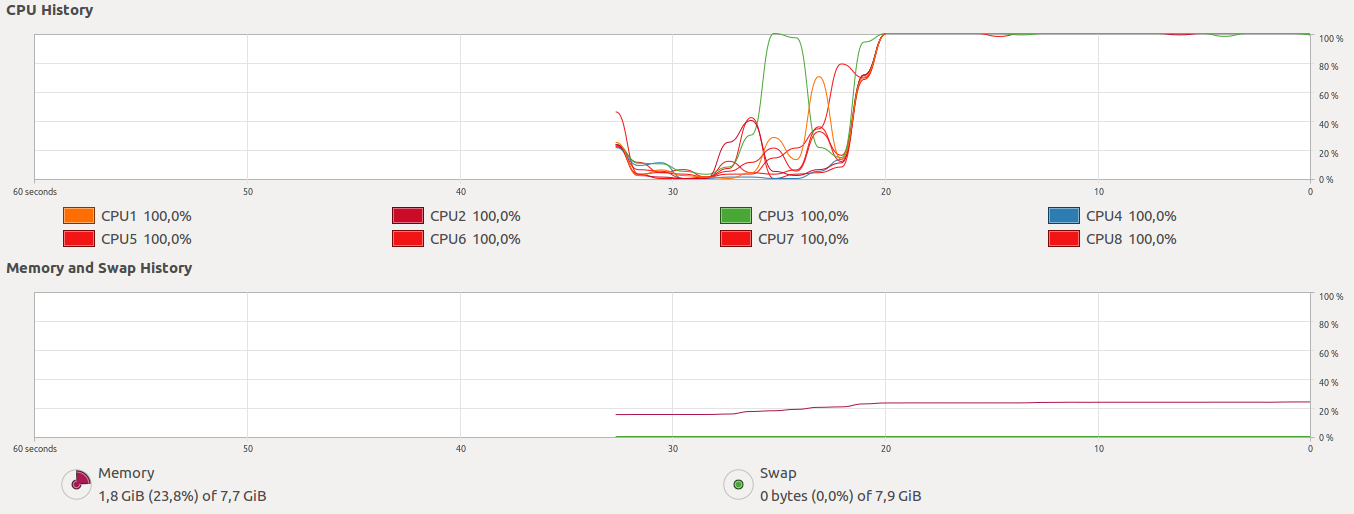
\includegraphics[width=\textwidth]{timeline0}\\
	En la parte de entrenamiento se calculan los codigos de cada una de las bandas del review, esta operacion se realiza paralelamente sobre el set de datos. Se particionan los set de datos en 8 particiones tal que haya un worker por nucleo del microprocesador. La operacion Non Lazy es un collect(), en la que se descargan los datos de la memoria de los Workers a la memoria de ejecucion del thread del interprete de python. \\ \\ 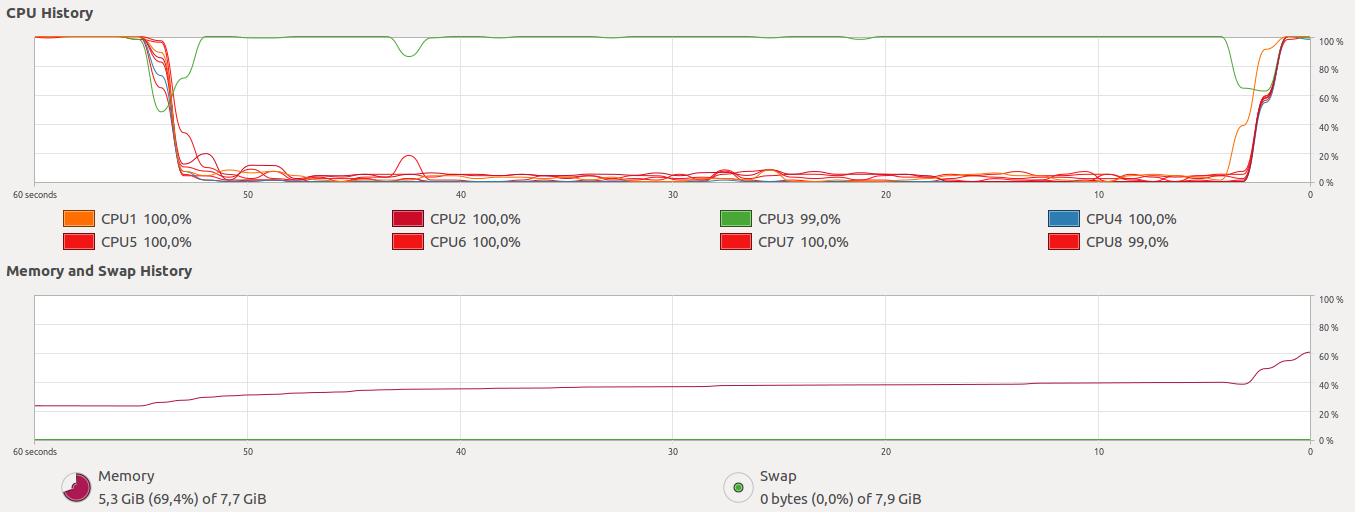
\includegraphics[width=\textwidth]{timeline1} \\ Con estos datos se construye un diccionario de python donde la clave es el codigo de hash asignado a cada banda y el valor una lista de todos los promedios que hay de entrenamiento para esa banda. Esta es la parte No Paralela del algoritmo. Una vez armado el diccionario se procede a predecir el set de datos. \\ \\ 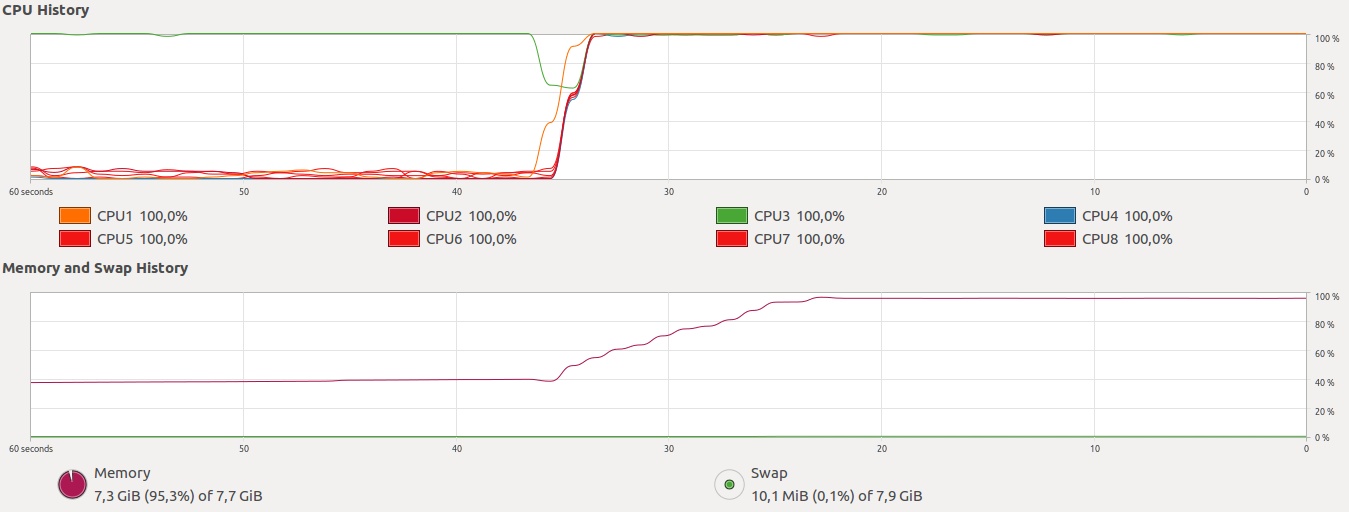
\includegraphics[width=\textwidth]{timeline2} \\ Luego en la etapa de prediccion, se carga un RDD con el set a predecir y se mapea al set de datos las instrucciones para calcular el score de cada review consultando en el diccionario los valores aprendidos. Se nos presentaron casos en los que las bandas de los minhashes de algunos reviews no encontraban ningun valor aprendido en el diccionario. En estos casos si estimaFaltantes = False, los reviews que no puedan ser calculados seran descartado. Si estimaFaltantes = True para todas las reviews se estima el valor medio de todos los valores posibles: 3. Es una aproximacion heuristica bastante pobre, pero se aplico con el fin de ver como afectaba el error cuadratico medio resultante.  \\ \\ 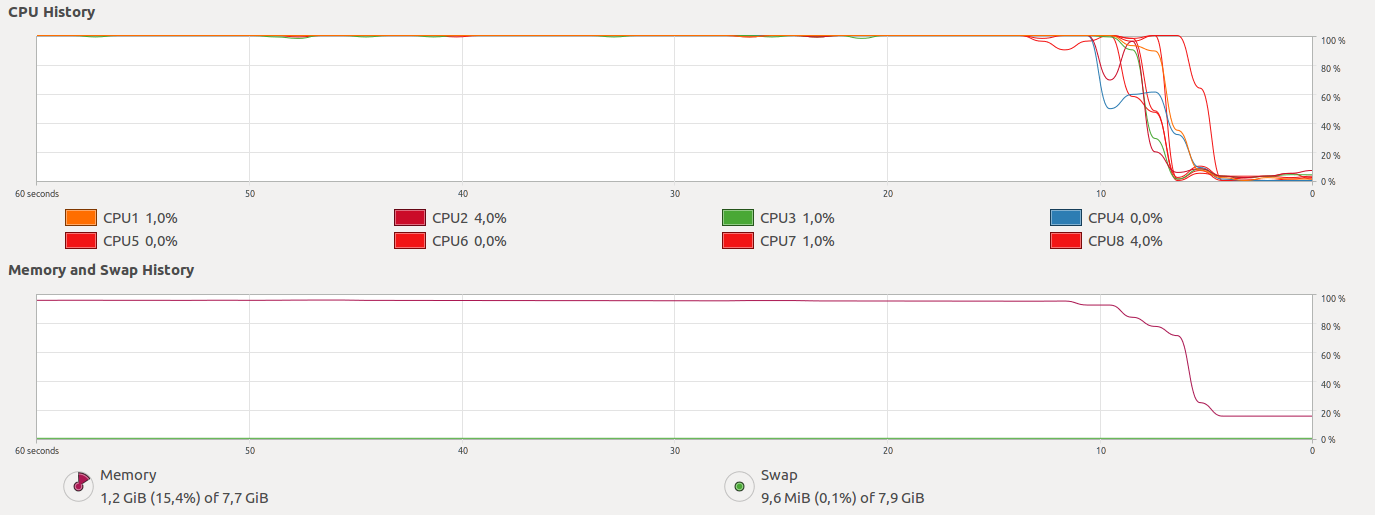
\includegraphics[width=\textwidth]{timeline3} \\ La siguiente operacion Non Lazy depende del flujo del programa. Si escribeScoresKaggle = True, se realiza un collect() y cada prediccion se escribe a un archivo csv. En el caso contrario, se mapean adicionales operaciones para calcular el error cuadratico medio donde la operacion Non Lazy es un reduce que acumula la diferencia al cuadrado de predictedScore y actualScore, y a su vez (como se reduce una tupla) se acumulan la cantidad de reviews para los cuales hubo prediccion.



	\subsection{Funciones de hashing}

	Con un claro objetivo en mente: predecir la mayor cantidad de reviews en la menor cantidad de tiempo (tambien consideramos elocuente no reinventar la rueda), decidimos utilizar la funcion de hashing provista por python: hash(). Esta funcion provee baja probabilidad de colision con una alta velocidad de computacion. Como utilizamos b Bandas de n cantidad de hashes cada una necesitamos b * n cantidad de diferentes funciones de hashing. Una manera eficiente y veloz de obtener una aproximacion semejante es de computar una unica vez b * n numeros semi-aleatorios. Para obtener las diferentes funciones de hashing con estos numeros semi-aleatorios probamos XORear o sumar el valor de hash(). La implementacion del XOR presento menor costo computacional (traducido en menor velocidad de procesamiento) y a su vez mejoro el error obtenido.
	
		
	\subsection{Variables e hyperparametros del algoritmo}

	maxint = sys.maxint\\
	Se utiliza para la primera comparacion del minhash. De esta manera siempre el primer minhash comparado sera menor a maxint.\\ \\

	bandas = 15 \\
	Cantidad de bandas. \\ \\
	
	hashesPorBanda = 1 \\
	Cantidad de funciones de hash por banda. Encontramos que al aumentar la cantidad de hashes por banda aumentaba significativamente la cantidad de reviews carecientes de score. Esto se da porque al tener dos hashes por banda aumenta la probabilidad de que las bandas no coincidan ya que se calculan a partir de dos hashes. \\ \\ 

	cantHashes = bandas * hashesPorBanda \\
	Cantidad de diferentes funciones de hashing. Encontramos que un valor superior a 15 generaba diccionarios demasiado grandes como para ser manejados en la memoria disponible \\ \\

	nGram = 15 \\
	Constante de los n-gramas. La implicancia directa de este hyperparametro se vio reflejada sobre la cantidad de reviews que el algoritmo no pudo predecir. Valores menores, daban menor contexto causando que las bandas muchas reviews hasheen a posiciones inexistentes del diccionario. Al aumentar la cantidad de caracteres de contexto a 20 o superior sucedia lo mismo. Los contextos eran tan amplios que los minhashes comenzaban a diferir notablemente entre los reviews, causando una menor tasa de recall. \\ \\

	xorHash = True \\
	Define si las variaciones de las funciones de hash se obtienen XOReando el numero random o sumandolo. A partir de investigacion se pudo concebir que la opcion mas acertada para obtener distintos valores de hash era aplicando la operacion XOR. Se pudo notar una leve mejoria en el error y a su vez en el tiempo de procesamiento. \\ \\

	shingleaWords = False \\
	Si shingleaWords == True, shinglea por palabras de lo contrario shinglea por caracter. \\ \\


	escribeScoresKaggle = False \\
	Si el flujo del programa es escribir resultados para el set de datos de kaggle, o para el set de datos grande. \\ \\


	estimaFaltantes = False \\
	Si estimaFaltantes  = True, aquellos reviews que no tuvieron ningun match para sus bandas se estiman con un valor de 3. De lo contrario se descartan. \\ \\
	
	lineasEnLearn = 300000 \\
	Cantidad de reviews para entrenar el algoritmo. \\ \\

	cantReviewsToPredict = 82680000 \\
	Cantidad de reviews para predecir. \\ \\

	hashDisplaces = [] \\
	En este arreglo se almacenan los numeros random para generar las distintas funcinoes de hashing. \\ \\

	valoresPorBanda = dict() \\
	En este diccionario se anotan los scores por clave de banda. \\ \\

	\section{Resultados sobre el dataset}
	Bandas: 15\\
	XOR: True\\
	Hashes por banda: 1\\
	Cantidad de hashes: 15\\
	Shinglea por caracteres con K-Grams: 15\\\\\\
	
	LINEAS EN EL LEARN: 100000\\
	CLAVES EN EL DICC: 1050230\\
	BANDAS CALCULADAS: 1500000\\
	REVIEWS A PREDECIR: 82680000\\
	REVIEWS CON SCORE: 72591094\\
	RELACION: 0.87797646\\
	PROMEDIO DE LOS CUADRADOS DE LAS DIFERENCIAS: 1.46986627444\\
	real	838m24.028s\\
	user	12m1.468s\\
	sys	1m56.160s\\\\
	
	
	LINEAS EN EL LEARN: 300000\\
	CLAVES EN EL DICC: 2878527\\
	BANDAS CALCULADAS: 4500000\\
	REVIEWS A PREDECIR: 82680000\\
	REVIEWS CON SCORE: 77461794\\
	RELACION: 0.93688672\\
	PROMEDIO DE LOS CUADRADOS DE LAS DIFERENCIAS: 1.37767813547\\
	real	907m22.183s\\
	user	16m48.616s\\
	sys	3m13.928s\\
	
	
	\section{Otras implementaciones descartadas}
	
	\subsection{Lideres y seguidores con Delta TFIDF}

	Otra opci\'{o}n que implementamos, en paralelo con LSH, fue aproximar KNN con lideres y seguidores, utilizando como m\'{e}trica una variante de TF-IDF (con BM25 y normalizando los datos), llamada Delta TF-IDF [10] utilizada para el an\'{a}lisis de sentimiento, para lo cual armamos diccionarios de palabras positivas y negativas, en lo cuales contabamos la frecuencia de cada palabra en los reviews positivos y negativos, consideramos positivos a los reviews de score 4 y 5, y negativos a los de score 1, 2 y 3. En este caso al procesar los datos quitamos todos los signos, las stopwords y no utilizamos ngramas. \\ \\
	 Descartamos esta idea porque era muy lenta al comparar el valor de delta TFIDF contra otro review, por lo tanto al comparar contra los lideres, y luego contra los seguidores del lider mas cercano se volvia muy lento el algoritmo al predecir, tardando en promedio 3 segundos por review.
	
	
	
	\begin{thebibliography}{99}
		\bibitem{INT06} Image-based recommendations on styles and substitutes. J. McAuley, C. Targett, J. Shi, A. van den Hengel. SIGIR, 2015
		\bibitem{INT06} Inferring networks of substitutable and complementary products. J. McAuley, R. Pandey, J. Leskovec. Knowledge Discovery and Data Mining, 2015
		\bibitem{INT06} LSH (Locality Sensitive Hashing, WikiPedia, https://en.wikipedia.org/wiki/Locality\-sensitive\_hashing
		\bibitem{INT06} Data Paralelism , WikiPedia, https://en.wikipedia.org/wiki/Data\_parallelism.
		\bibitem{INT06} KNN (K Vecinos mas cercanos), WikiPedia, https://es.wikipedia.org/wiki/K\-vecinos\_m\%C3\%A1s\_cercano
		\bibitem{INT06} Apache Spark, WikiPedia,https://en.wikipedia.org/wiki/Apache\_Spark
		\bibitem{INT06} Programacion neurolinguistica, https://es.wikipedia.org/wikiProgramaci\%C3\%B3n\_neuroling\%C3\%BC\%C3\%ADstica
		\bibitem{INT06} Apunte oficial de la materia, Luis Argerich
		\bibitem{INT06} CONFIGURACION SPARK https://blog.cloudera.com/blog/2015/03/how-to-tune-your-apache-spark-jobs-part-2/
		\bibitem{INT06} Delta TF-IDF http://ebiquity.umbc.edu/_file_directory_/papers/446.pdf

	\end{thebibliography}
	
\end{document}
